\documentclass[a4paper, 12pt]{scrartcl}
\usepackage[T1]{fontenc}
\usepackage[utf8]{inputenc}
\usepackage[ngerman]{babel}

\usepackage{paralist}
\usepackage{multicol}

\usepackage{amssymb}
\usepackage{amsmath}
\usepackage{pifont}

\usepackage{listings}
\usepackage{color}

\usepackage{enumitem} % used for letters i, ii, iii... in enumerate

\usepackage{graphicx}

%setup
\author{Jakob Otto\\
	\texttt{2266015} \and Martin Beckmann\\
	\texttt{2324916}}

\title{VS-Aufgabe 1\\
       Abgabe}

% setting locales
\usepackage[utf8]{inputenc}
\usepackage[T1]{fontenc}
\usepackage[ngerman]{babel}
\usepackage{lmodern}
\usepackage[locale=DE,list-final-separator={ oder },range-phrase={ bis },scientific-notation=false,group-digits=integer]{siunitx}

% package includes
\usepackage{xcolor}
\usepackage{listings}

%listing setup
\definecolor{pblue}{rgb}{0.13,0.13,1}
\definecolor{pgreen}{rgb}{0,0.5,0}
\definecolor{pred}{rgb}{0.9,0,0}
\definecolor{pgrey}{rgb}{0.46,0.45,0.48}
\definecolor{javared}{rgb}{0.6,0,0} % for strings
\definecolor{javagreen}{rgb}{0.25,0.5,0.35} % comments
\definecolor{javapurple}{rgb}{0.5,0,0.35} % keywords
\definecolor{javadocblue}{rgb}{0.25,0.35,0.75} % javadoc

\lstset{language=java,
	basicstyle=\ttfamily,
	keywordstyle=\color{javapurple}\bfseries,
	stringstyle=\color{javared},
	commentstyle=\color{javagreen},
	morecomment=[s][\color{javadocblue}]{/**}{*/},
	numbers=left,
	numberstyle=\tiny\color{black},
	stepnumber=2,
	numbersep=10pt,
	tabsize=2,
	showspaces=false,
	showstringspaces=false
}


\begin{document}
\maketitle
\newpage
	
\section{Aufgabe}
In diesem Praktikumstermin sollte eine verteile Client-Server-Anwendung programmiert werden. Dabei wurde auf Verteilungstranzparenz, Interoperabilität und eine definierte Fehlertoleranz geachtet.

\subsection{Verteilungstransparenz/Interoperabilität}
Die Verteilungstranzparenz wird gewährleistet, indem der Server von der Klasse Remote erbt. Somit ist seine Nutzung in einem verteilten System fast identisch mit seiner Nutzung in einem lokalen System. Der einzige Unterschied liegt in der Beschaffung einer Referenz auf den Server im Client. Dieser würde über einen Aufruf Naming.lookup("MessageService") erfolgen. Dieser Aufruf liefert eine Remote-Referenz mit der anschließend gearbeitet werden kann.
Die Interoperabilität wird durch ein einheitliches Interface sichergestellt. Wenn sich jede Implementation des Servers an das Interface aus der Aufgabenstellung hält, können alle Clients mit diesen Servern kommunizieren.

\subsection{Fehlertoleranz/Semantiken}
Die definierte Fehlertoleranz wird erreicht, indem die korrekte Fehlersemantik aus der Aufgabenspezifikation implementiert wird.

Die Methode \lstinline|nextMessage(String clientId)| vom Server soll eine \glqq{}at-most-once\grqq{} Fehlersemantik implementieren. Das heißt, dass der Client mehrere Anfragen stellen kann und der Server Duplikate dieser Anfragen filtert. Die angefragte Nachricht wird dann maximal \textbf{ein mal} ausgeliefert.

Das Senden einer Nachricht eines Clients soll die \glqq{}at-least-once\grqq{} Fehlersemantik implementieren. Dabei stellt der Client so lange Anfragen, bis der Server den Erhalt der Nachricht mit einem Acknowledgement bestätigt. Es ist also sichergestellt, dass der Server die Nachricht \textbf{mindestens} ein mal erhält -- es ist aber nicht ausgeschlossen, dass die Nachricht öfter dort eintrifft. Der Server sollte dies erkennen und die eintreffenden Nachrichten entsprechend filtern.

Das Abholen aller verfügbaren Nachrichten soll mit der Fehlersemantik \glqq{}maybe\grqq{} implementiert werden. Diese Fehlersemantik kommt der lokalen Programmierung am nächsten. Anfragen werden genau einmal gesendet und Verlust von Nachrichten wird in kauf genommen. Beim Verlust von Daten wird die Anfrage nicht noch ein mal gesendet.

Zusätzlich sollen Clients für ein konfigurierbares Zeitintervall $s$ robust gegen Serverausfälle sein. Das wird erreicht indem konstant wieder auftretende Fehler vom Server erst nach s Sekunden als Serverausfall interpretiert werden. Beim Ausfall des Servers wird ein reconnect versucht.

Zu den Implementierungen dieser Semantiken mehr im Absatz \glqq{}Implementation\grqq{}

\section{Implementation}
Das Verteilte Client-Server-Programm wurde mit Hilfe des Java-RMI realisiert. Die RMI-Schnittstelle kapselt bereits das generieren von Stub-Objekten, sowie den Verbindungsaufbau und das aufrufen von Methoden auf den sogenannten \glqq{}Remote-Objekten\grqq{}. 

\subsection{MessageServer} Die Klasse \lstinline|MessageServer| hat für das realisieren der remote-method-invocation die Klasse Remote extended. Dadurch war es möglich das \lstinline|MessageServer|-Objekt mit Hilfe eines Registry-eintrags auf verschiedene Rechner zu verteilen und an diesem dann Methoden aufzurufen. Die dafür nötigen Schritte waren:
\begin{enumerate}
	\item starten/holen einer Registry
	\item erzeugen eines \lstinline|MessageServer| Objekts
	\item exportieren dieses Objekts per Aufruf von \lstinline|registry.rebind("identifier", obj);|
\end{enumerate}
Danach war es möglich einen Stub dieses Objekts zu erhalten und darüber mit diesem zu kommunizieren.
Der Server hatte außerdem noch die Aufgabe die ClientConnections zu managen. Hierzu wurde eine Klasse \lstinline|ClientConnection| implementiert, welche den letzten Zugriff auf den Server und die letzte erhaltene Nachricht enthielt. Dadurch konnte gespeichert werden, welcher Client, welche Nachrichten schon erhalten hat und außerdem ein timeout realisiert werden. Nach ablauf des Timeouts wurde der Client \glqq{}vollständig\grqq{} vergessen.

\subsection{MessageClient}
Der \lstinline|MessageClient| hat in unserem Fall den Zugriff auf den \lstinline|MessageServer| gekapselt. Die Aufgabe dieser Klasse war, ein Stub-Objekt des Servers aus der Registry zu erhalten und auf die beiden Methoden \lstinline|String nextMessage(String clientID)| und \lstinline|void newMessage(String clientID, String message)| geeignet zuzureifen.

\subsection{Implementierung der Fehlersemantiken}
\subsection{maybe}
Für diese Fehlersemantik musste kein besonderer Implementierungsaufwand betrieben werden, da die Anfrage beliebig oft gesendet und bearbeitet werden durfte. Verlorene Anfragen, oder duplikate dieser Anfragen mussten also nicht besonders betrachtet werden.

\subsection{at-most-once}
Für diese Fehlersemantik musste etwas mehr implementierungsaufwand erfolgen. Da eine Message \textbf{maximal} einmal ausgeliefert werden, aber die Anfrage für diese beliebig oft erfolgen durfte, mussten die Einzelnen Anfragen Serverseitig gespeichert werden. Hierfür wurde eine Klasse \lstinline|Request| implementiert, welche die ClientID und die Message enthielt. Bei jeden Request wurde ein soches Objekt erzeugt und in einem Set gespeichert. Bei einem weiteren \textbf{identischen} Request kann dieser dem \glqq{}requestSet\grqq{} nicht hinzugefügt werden und der Request wird ignoriert.

\subsection{at-least-once}
Für diese Fehlersemantik wurde eine loop implementiert, welche das Senden einer Nachricht wiederholt, falls das entsprechende ACK des Servers nicht eingetroffen ist. 
Sobald die Anfrage verloren gegangen ist, wird durch das Java-RMI eine Exception ausgelöst, welche das mislingen des Requests Signalisiert. Falls eine solche Exception aufgetreten ist, sollte der Client eine Zeit $s$ warten und den Request wiederholen.


\newpage
\section{Tests}
Die hier nachfolgend erläuterten Tests sollen vorrangig testen, ob die Fehlersemantiken für die Anwendung korrekt implementiert wurden.
Da die richtige Implementation der Fehlersemantiken vom Client implementiert werden müssen, wurde eine weitere Serverklasse geschrieben, welche das vorgegebene Interface implementiert. Somit kann der Client normal mit dem Server sprechen, und zeitgleich können wir sicherstellen, dass gewisse problematische Situationen auftreten um das Verhalten des Clients zu prüfen.
Da Fehlersemantiken erst eine Rolle spielen, wenn Anfragen zum Server verloren werden können, müssen wir dies also simulieren. Das wurde erreicht, indem der Server jeweils zählt wie viele \glqq{}nextMessage\grqq{}- und \glqq{}newMessage\grqq{}-Anfragen er bereits bekommen hat, und alle n Anfragen mit einer RemoteException direkt quittiert. Da der Client nicht unterscheiden kann warum die Exception geworfen wurde, muss die Fehlerbehandlung die gleiche sein, als wäre die Anfrage durch eine schlechte Verbindung verloren worden.
Wenn die Fehlersemantiken korrekt implementiert wurden, erwarten wir, dass trotz schlechter Verbindung alle Nachrichten erfolgreich an den Server gesendet werden (\glqq{}at-least-once\grqq{}), jedoch nicht immer alle Nachrichten erfolgreich vom Server an die Clients gesendet werden kann (\glqq{}maybe\grqq{}).
Der genaue Testablauf besteht daraus, dass der Nutzer die Nachrichten \glqq{}1\grqq{}, \glqq{}2\grqq{}, \glqq{}3\grqq{}... sendet. Zu erwarten ist, dass die Nachrichten nicht unmittelbar, sondern erst nach kurzer Zeit aus dem Textfeld verschwinden. Das liegt daran, dass der Client eine gewisse Zeit wartet bevor eine fehlgeschlagene Anfrage erneut an den Server senden.
Nachdem ein paar Nachrichten gesendet wurden, versucht man die Nachrichten vom Server ausliefern zu lassen. Aufgrund der simulierten schlechten Verbindung zum Server werden manche Anfragen nicht korrekt überliefert. Das führt dazu, dass der Nutzer manuell mehrere Male die nächste Nachricht anfragen muss bis diese auch in der GUI erscheint. Wenn man die Nachrichten häufig genug angefragt hat, stehen sie anschließend alle, vom Nutzer gesendeten, Texte in der oberen Textbox.
Somit ist zu erkennen, dass tatsächlich alle Nachrichten erfolgreich an den Server ausgeliefert werden und Nachrichten \glqq{}maybe\grqq{} vom Server geholt werden.

\newpage
\section{wireshark}
Im Zuge des testens des geschriebenen Programms, wurde der Traffic zwischen Client und Server mit Hilfe von wireshark aufgezeichnet. Im folgenden werden dert Traffic bei Verbindungsaufbau, senden von Nachrichten und empfangen von Nachrichten festgehalten.

\subsection{Verbindungsaufbau}
\begin{center}
	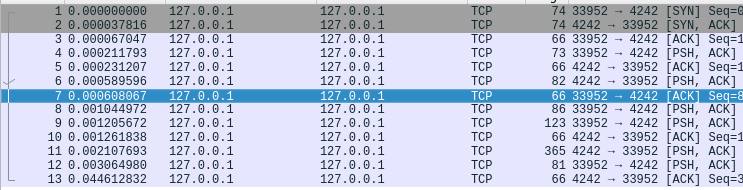
\includegraphics[width=\textwidth]{connect.png}
\end{center}
\begin{center}
	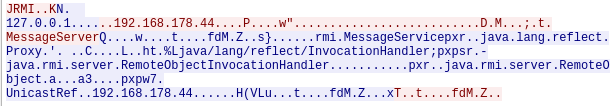
\includegraphics[width=\textwidth]{connect_data.png}
\end{center}

\subsection{senden von Nachrichten}
\begin{center}
	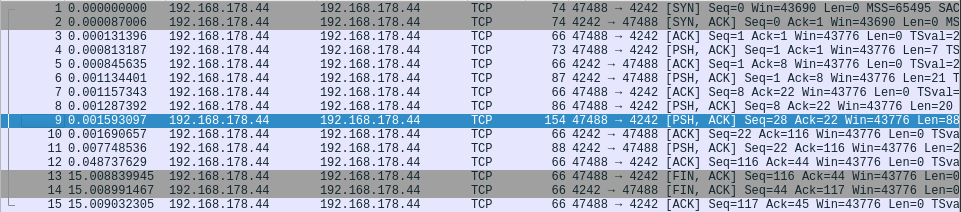
\includegraphics[width=\textwidth]{senden.png}
\end{center}
\begin{center}
	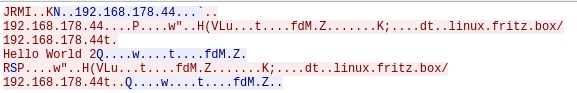
\includegraphics[width=\textwidth]{senden_data.png}
\end{center}

\subsection{empfangen von Nachrichten}
\begin{center}
	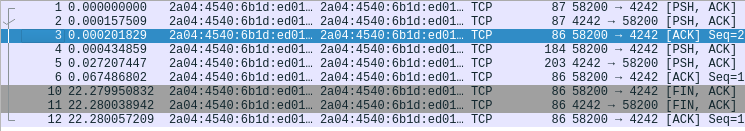
\includegraphics[width=\textwidth]{empfangen.png}
\end{center}
\begin{center}
	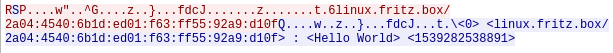
\includegraphics[width=\textwidth]{empfangen_data.png}
\end{center}
\newpage
\section{Klassen/Interfaces}
\subsection{MessageService}
\begin{lstlisting}
public interface MessageService extends Remote {
	String nextMessage(String clientID) throws RemoteException;
	void newMessage(String clientID, String message) throws RemoteException;
}
\end{lstlisting}

\subsection{ClientConnection}
\begin{lstlisting}
public class ClientConnection {
    int lastMessageID;
	long timeStamp;
}
\end{lstlisting}

\subsection{MessageServer}
\begin{lstlisting}
public class MessageServer implements MessageService {
private static final int MAX_QUEUE_SIZE = 30;
private static final int MAX_CONN_AGE_MILLISECONDS = 30_000;
private static final int PORT = 4242;
private List<Message> deliveryQueue;
private Map<String, ClientConnection> connections;
private Set<Request> requests;

/**
* gets the next message from the delivery queue
* @param clientID the clientID of the requesting client
* @return the next message from the queue or null if no further message is present
*/
public String nextMessage(final String clientID);

/**
* takes a new message and places it into the delivery queue
* @param clientID the clientID of the sender
* @param message the message that is delivered
*/
public void newMessage(final String clientID, final String message);

/**
* manages creating and updating of the ClientConnection objects
* @param clientID the ID of the client
* @return the Object that was created or updated
*/
private ClientConnection manageConnection(final String clientID);

/**
* keeps server alive and keeps client connections sorted.
* when a client timed out, this routine 'forgets' about that client and removes its
* ClientConnection Object.
*/
public void run();

/**
* publishes the MessageServer Object and starts the run method
* @param args arguments for the program
*/
public static void main(String... args);
\end{lstlisting}

\subsection{MessageClient}
\begin{lstlisting}
public class MessageClient implements IModel {
private static final String HOST = "localhost";
private static final int PORT = 4242;
private static final int SERVER_TIMEOUT_SECONDS = 2;
private final String clientID;
private MessageService ms;

/**
* sends the given message to the server. implements a 'at least once' semantic
* @param message the message that should be sent to the server
*/
@Override
public void sendMessage(String message);

/**
* receives all pending messages at once.
* @return a list containing all received messages
*/
@Override
public String getAllMessages();

/**
* gets the next message from the server. implements a 'at most once' semantic
* @return the message that was received or null if no further messages are present
*/
@Override
public String getMessage();
\end{lstlisting}

\subsection{Message}
\begin{lstlisting}
public class Message {
	String message;
	int id;
	String client_ID;
	long timestamp;
}
\end{lstlisting}

\subsection{Request}
\begin{lstlisting}
public class Request {
Request (String clientID, String message) {
	private String clientID;
	private String message;
}
\end{lstlisting}

\newpage	
\section{Quellen}
https://vsis-www.informatik.uni-hamburg.de/oldServer/teaching/ws-11.12/vis/folien/06a-RPC.pdf Seite 45-Ende
\end{document}

